\chapter{Habilidades.}
%=============================================================
	\section{Cuchillas de obsidiana} \label{hab.CuchObs}	
		\subsection{Descripción}
		El enemigo lanza pequeños círculos rojos en dirección horizontal que dañan al jugador. Los disparos salen de la parte frontal del enemigo.
		\subsection{Portador}
		Armadillo (ver apartado \ref{per:armadillo})
		\subsection{Esquema}

%============================================================
		\section{Nombre: Disparo rojo.} \label{hab.disparoR}
		\subsubsection{Descripción}
		El enemigo lanza pequeños círculos rojos en dirección horizontal que dañan al jugador. Los disparos salen de la parte frontal del enemigo.
		\subsubsection{Portador}
		Fantasma rojo. Ver \ref{per.fantasmaR}.
		\subsubsection{Esquema}
		Ver figura \ref{fig:disparoR}.
		\begin{figure}
			\centering
			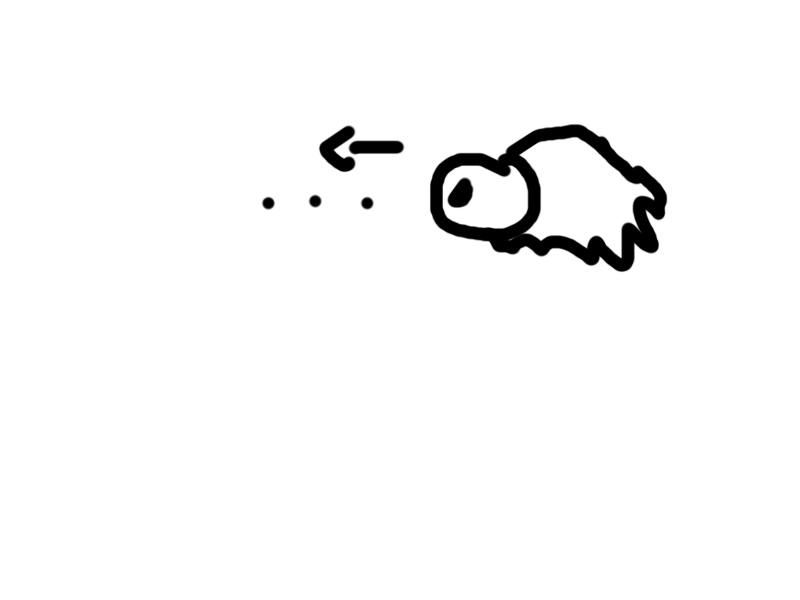
\includegraphics[height=0.2 \textheight]{Imagenes/disparoR}
			\caption{Disparo rojo.}
			\label{fig:disparoR}
		\end{figure}
		
%============================================================
	\section{Nombre: Flotar en vertical.} \label{hab.flotarV}
		\subsection{Descripción}
		El enemigo se desplaza sobre el piso, moviéndose de manera vertical. Llega a determinada altura y vuelve a bajar al piso.
		\subsection{Portador}
		Fantasma rojo. Ver \ref{per.fantasmaR}.
		\subsection{Esquema}
		Ver figura \ref{fig:flotarV}.
		\begin{figure}
			\centering
			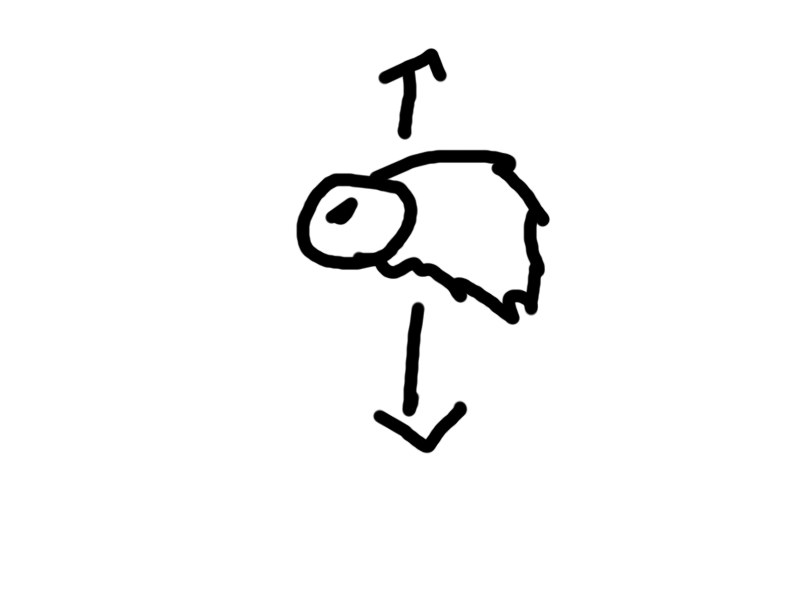
\includegraphics[height=0.2 \textheight]{Imagenes/flotarV}
			\caption{Flotar en vertical.}
			\label{fig:flotarV}
		\end{figure}
		%============================================================
	\section{Nombre: Embestida.} \label{hab.embestida}
		\subsection{Descripción}
		El enemigo aumenta su velocidad mientras se desplaza de arriba hacia abajo en diagonal.
		\subsection{Portador}
		Fantasma morado. Ver \ref{per.fantasmaM}.
		\subsection{Esquema}
		Ver figura \ref{fig:embestida}.
		\begin{figure}
			\centering
			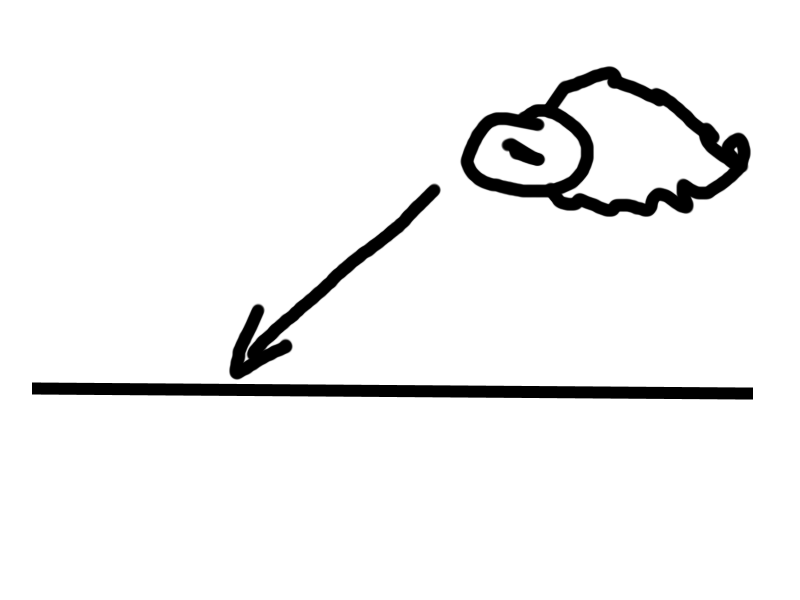
\includegraphics[height=0.2 \textheight]{Imagenes/embestida}
			\caption{Embestida.}
			\label{fig:embestida}
		\end{figure}

%============================================================
	\section{Nombre: Flotar en triángulo.} \label{hab.flotarT}
		\subsection{Descripción}
		El enemigo se mueve por tres diferentes nodos, dibujando un triángulo. Al final regresa al primer nodo.
		\subsection{Portador}
		Fantasma morado. Ver \ref{per.fantasmaM}.
		\subsection{Esquema}
		Ver figura \ref{fig:flotarT}.
		\begin{figure}
			\centering
			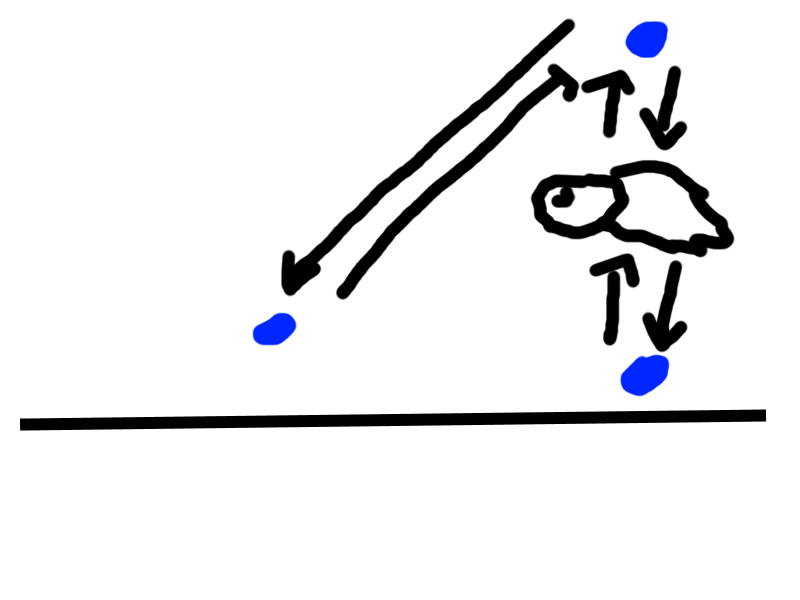
\includegraphics[height=0.2 \textheight]{Imagenes/flotarT}
			\caption{Flotar en triángulo.}
			\label{fig:flotarT}
		\end{figure}

%============================================================
	\section{Nombre: Rapto.} \label{hab.rapto}
		\subsection{Descripción}
		El enemigo se mueve hacia la posición del jugador, lanzándose de su posición hacia abajo con una desviación curva.
		\subsection{Portador}
		Zopilote. Ver \ref{per.zopilote}.
		\subsection{Esquema}
		Ver figura \ref{fig:rapto}.
		\begin{figure}
			\centering
			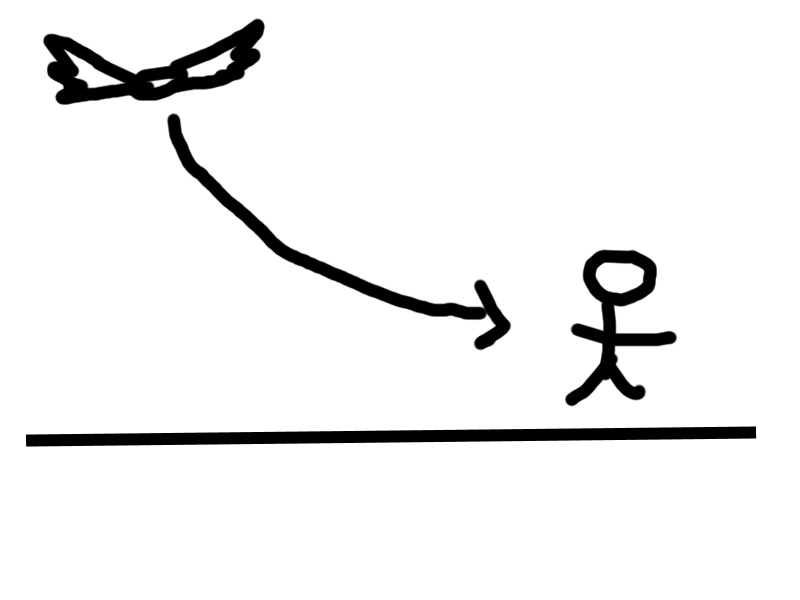
\includegraphics[height=0.2 \textheight]{Imagenes/rapto}
			\caption{Zopilote.}
			\label{fig:rapto}
		\end{figure}

%============================================================
	\section{Nombre: Zopilotear.} \label{hab.zopilotear}
		\subsection{Descripción}
		El enemigo se mueve de manera circular por sobre el piso.
		\subsection{Portador}
		Zopilote. Ver \ref{per.zopilote}.
		\subsection{Esquema}
		Ver figura \ref{fig:zopilotear}.
		\begin{figure}
			\centering
			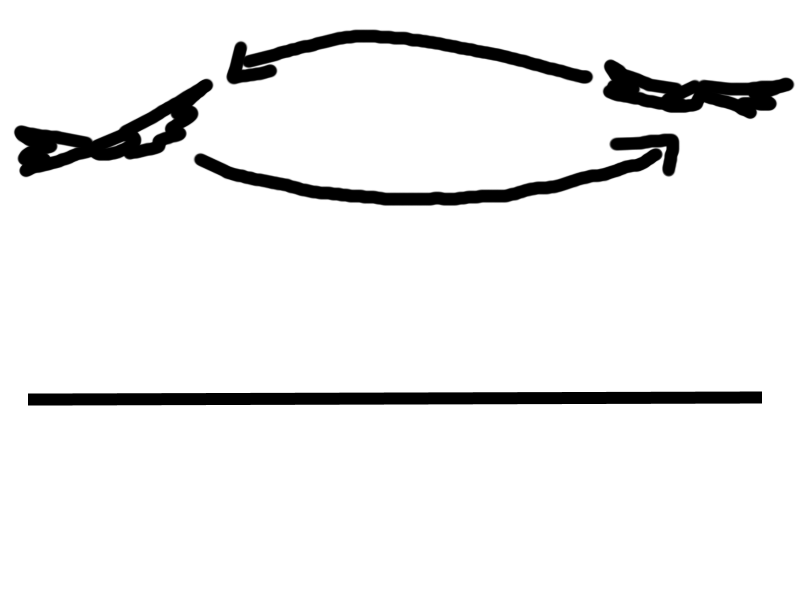
\includegraphics[height=0.2 \textheight]{Imagenes/zopilotear}
			\caption{Zopilotear.}
			\label{fig:zopilotear}
		\end{figure}

%============================================================
			\section{Nombre: Zarpazo.} \label{hab.zarpazo}
			\subsection{Descripción}
			El enemigo con sus garras ataca al jugador.
			\subsection{Portador}
			Jaguar. Ver \ref{per.jaguar}.
			\subsection{Esquema}
			Ver figura \ref{fig:zarpazo}.
			\begin{figure}
				\centering
				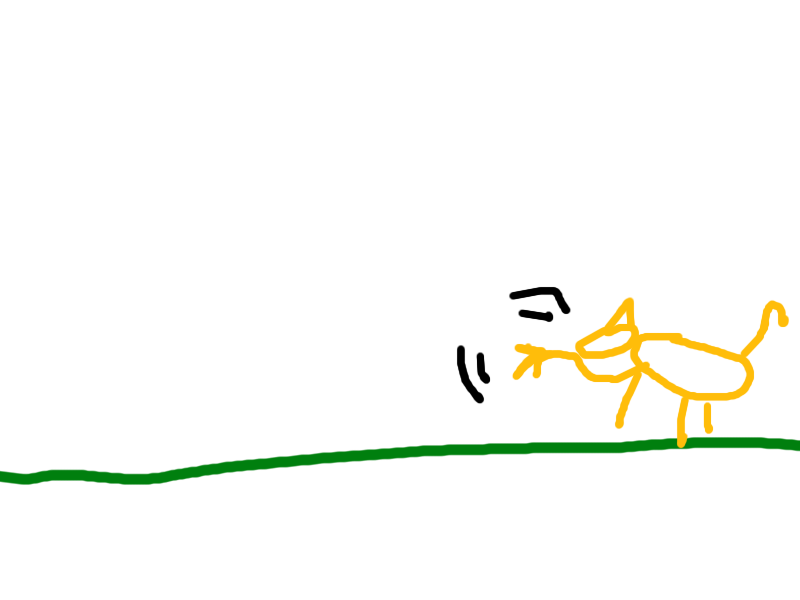
\includegraphics[height=0.2 \textheight]{Imagenes/zarpazo}
				\caption{Zarpazo.}
				\label{fig:zarpazo}
			\end{figure}
			
			%============================================================
\section{Nombre: Disparo de tonalli.}\label{hab.disparoT}
\subsection{Descripción}
Con ayuda de la caracola permite a su portador disparar tonalli.
\subsection{Portador}
Malinalli
\subsection{Esquema}
			Ver figura \ref{fig:disparoT}.
			\begin{figure}
				\centering
				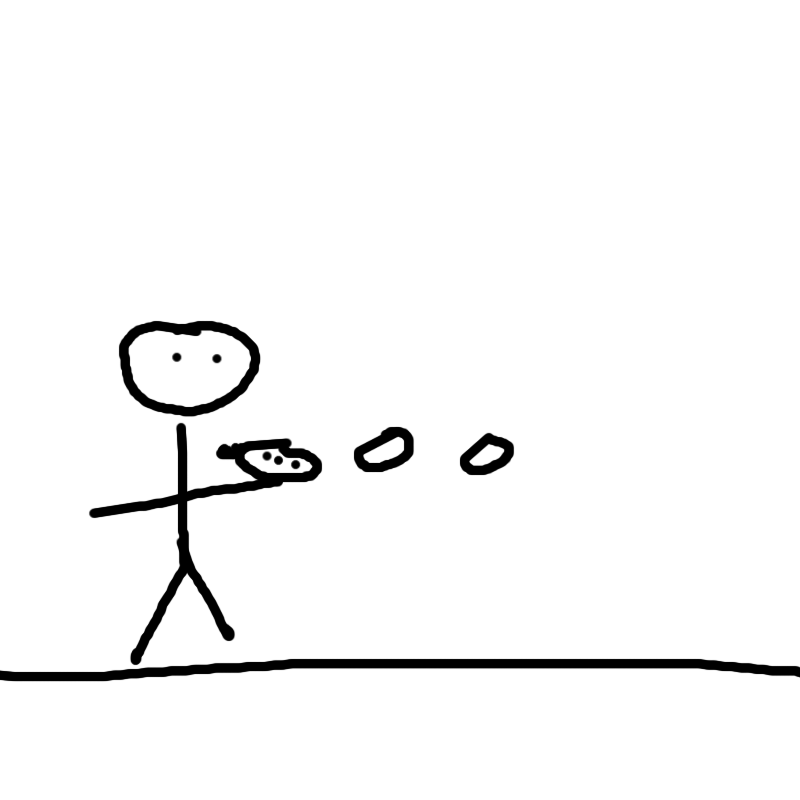
\includegraphics[height=0.2 \textheight]{Imagenes/disparoT}
				\caption{Disparo de tonalli por el jugador.}
				\label{fig:disparoT}
			\end{figure}
			
%============================================================
\section{Nombre: Zambullida.}\label{hab.zambullida}
\subsection{Descripción}
Zochitónal se sumerge en el río, dejando solo en la superficie parte de su espalda; procediendo a nadar a gran velocidad de un lado a otro para embestir a sus enemigos.  
\subsection{Portador}
Zochitónal
\subsection{Esquema}
			Ver figura \ref{fig:zambullida}.
			\begin{figure}
				\centering
				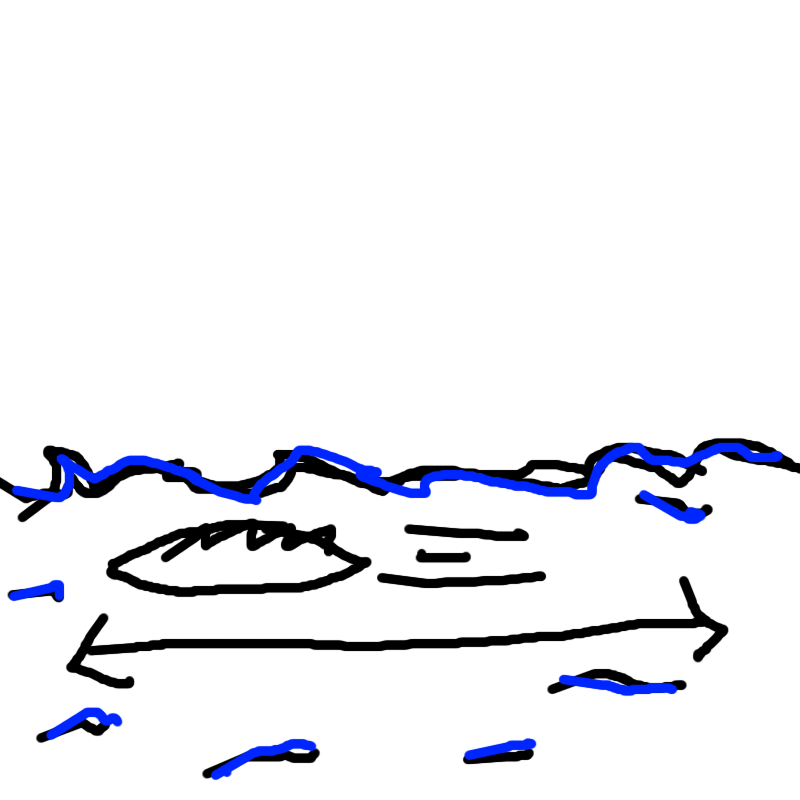
\includegraphics[height=0.2 \textheight]{Imagenes/zambullida}
				\caption{Zambullida.}
				\label{fig:zambullida}
			\end{figure}
%============================================================
\section{Nombre: Burbujas.}\label{hab.burbujas}
\subsection{Descripción}
Zochitónal dispara burbujas que seguirán al jugador por un tiempo.  
\subsection{Portador}
Zochitónal
\subsection{Esquema}
			Ver figura \ref{fig:burbujas}.
			\begin{figure}
				\centering
				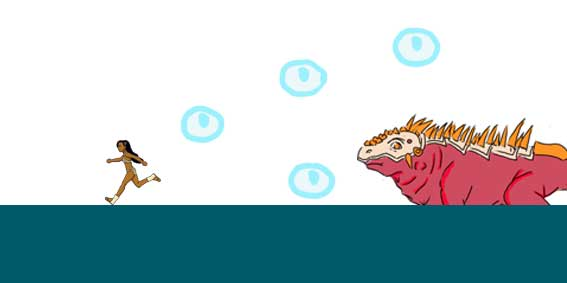
\includegraphics[height=0.2 \textheight]{Imagenes/burbujas}
				\caption{Burbujas.}
				\label{fig:burbujas}
			\end{figure}

%============================================================
\section{Nombre: Coraza.}\label{hab.coraza}
\subsection{Descripción}
Esta habilidad permite crear una coraza de piedra protegiendo a su portador de ataques enemigos sacrificando velocidad de movimiento.  
\subsection{Portador}
Tepeyóllotl.
\subsection{Esquema}
			Ver figura \ref{fig:coraza}.
			\begin{figure}
				\centering
				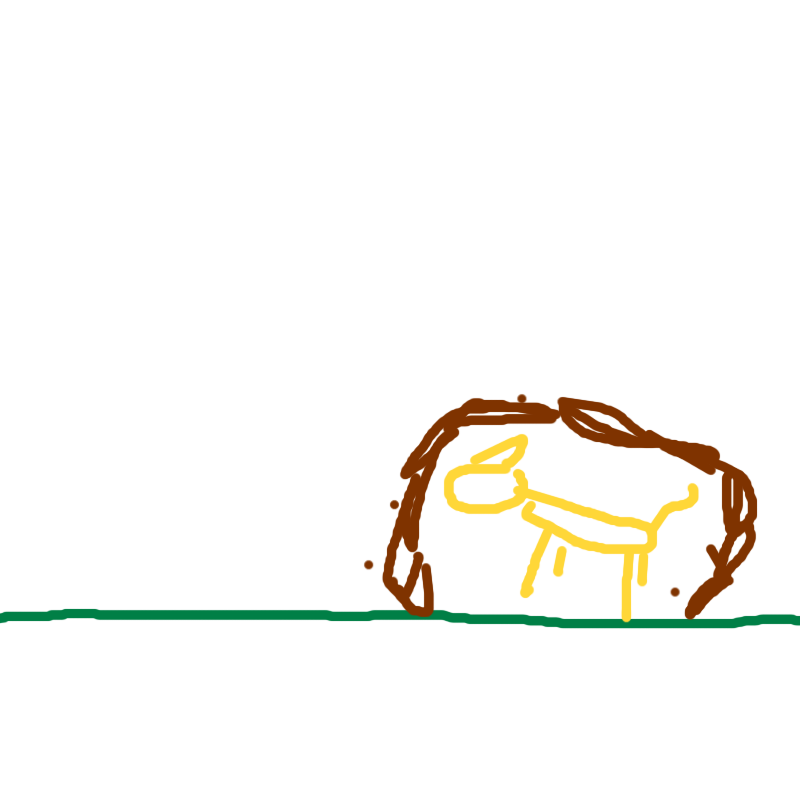
\includegraphics[height=0.2 \textheight]{Imagenes/coraza}
				\caption{Coraza.}
				\label{fig:coraza}
			\end{figure}
%============================================================
\section{Nombre: Impacto.} \label{hab.impacto}
\subsection{Descripción}
Realiza un salto, provocando al aterrizaje una onda de piedras en el suelo.
\subsection{Portador}
Tepeyóllotl.
\subsection{Esquema}

%============================================================
\section{Nombre de la habilidad: Luvia de rocas.} \label{hab.LLuviaRocas}
\subsection{Descripción}
Con un poderoso rugido provoca una avalancha de rocas. 
\subsection{Portador}
Tepeyóllotl.
\subsection{Esquema}
			Ver figura \ref{fig:lluviaR}.
			\begin{figure}
				\centering
				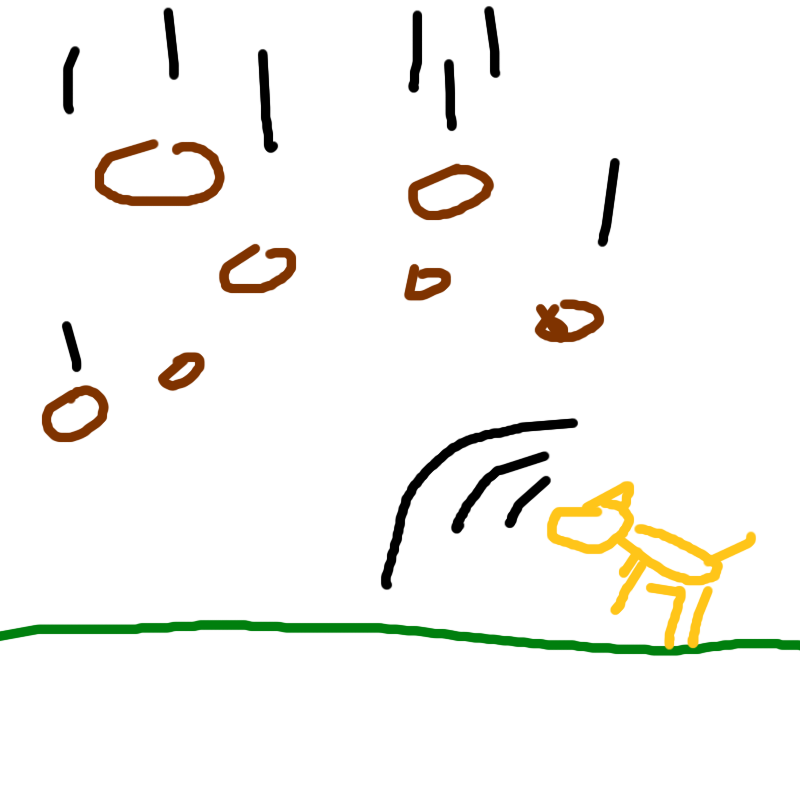
\includegraphics[height=0.2 \textheight]{Imagenes/lluviaR}
				\caption{Lluvia de rocas.}
				\label{fig:lluviaR}
			\end{figure}
			
%============================================================
\section{Nombre: Rugido aturdidor.}\label{hab.RugAtur}
\subsection{Descripción}
Poderoso rugido provoca una de continuo echo que inmoviliza a al enemigo, Tepeyóllotl solo puede usar esta habilidad cuando no usa la coraza. 
\subsection{Portador}
Tepeyóllotl. 
\subsection{Esquema}
			Ver figura \ref{fig:rugido}.
			\begin{figure}
				\centering
				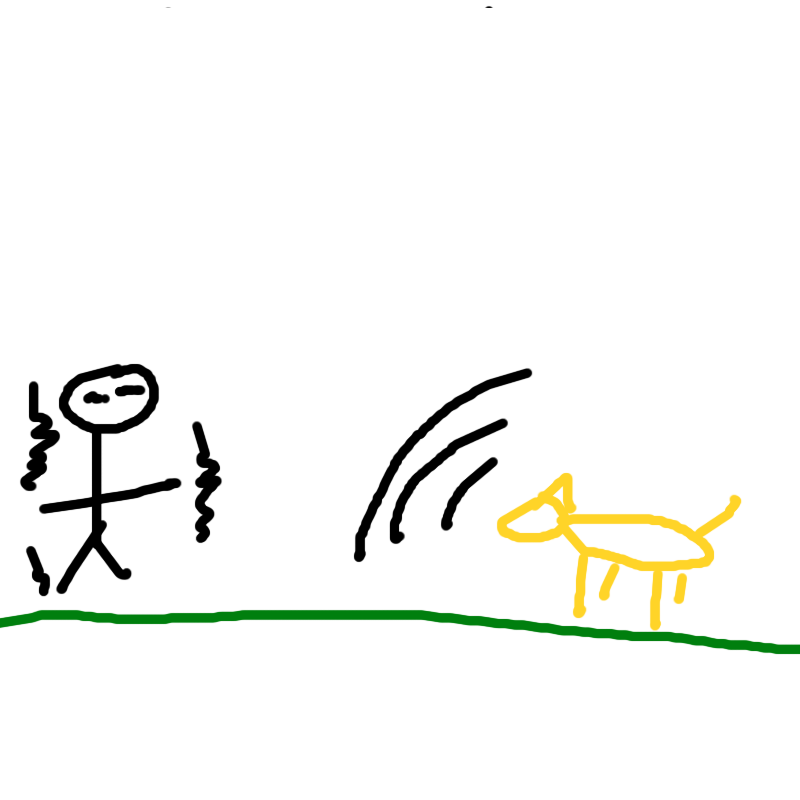
\includegraphics[height=0.2 \textheight]{Imagenes/rugido}
				\caption{Rugido aturdidor.}
				\label{fig:rugido}
			\end{figure}
			
%============================================================
\section{Nombre: Circulo de fuego.} \label{hab.CirFue}
\subsection{Descripción}
Itzpápalotl se eleva en el aire y se rodea a sí misma con fuego, este ataque sera usado cuando el jugador se encuentre junto a ella.
\subsection{Portador}
Itzpápalotl. 
\subsection{Esquema}
			Ver figura \ref{fig:circuloF}.
			\begin{figure}
				\centering
				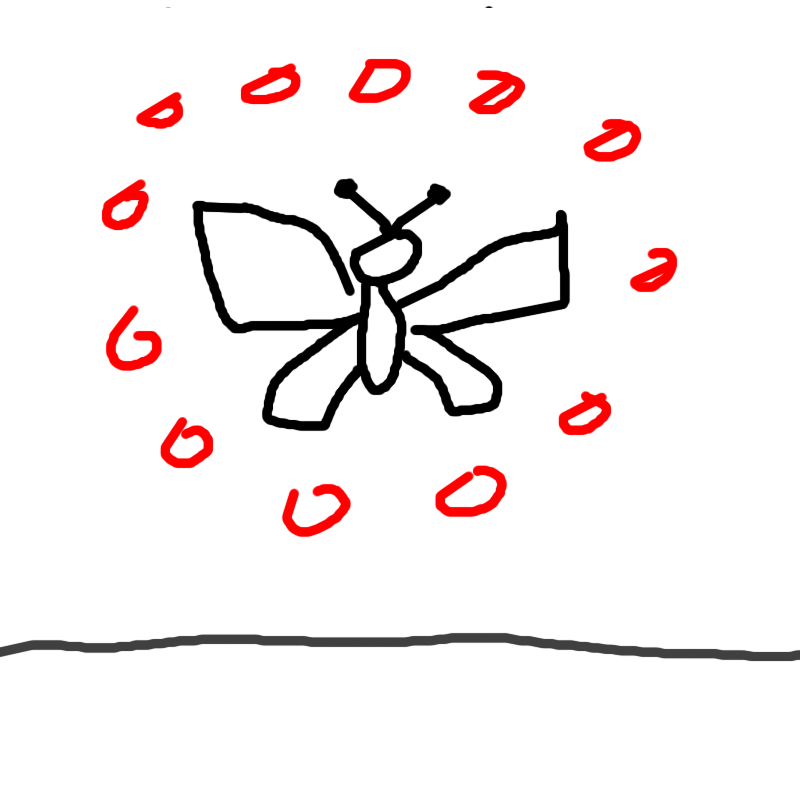
\includegraphics[height=0.2 \textheight]{Imagenes/circuloF}
				\caption{Círculo de fuego.}
				\label{fig:circuloF}
			\end{figure}
			
%============================================================
\section{Nombre: Embestida aerea.}\label{hab.EmbesAer}
\subsection{Descripción}
Itzpápalotl usara este ataque cuando este lejos del jugador. Itzpápalotl saltar y en el aire se lanza contra el enemigo en diagonal.
\subsection{Portador}
Itzpápalotl.
\subsection{Esquema}
			Ver figura \ref{fig:embestidaA}.
			\begin{figure}
				\centering
				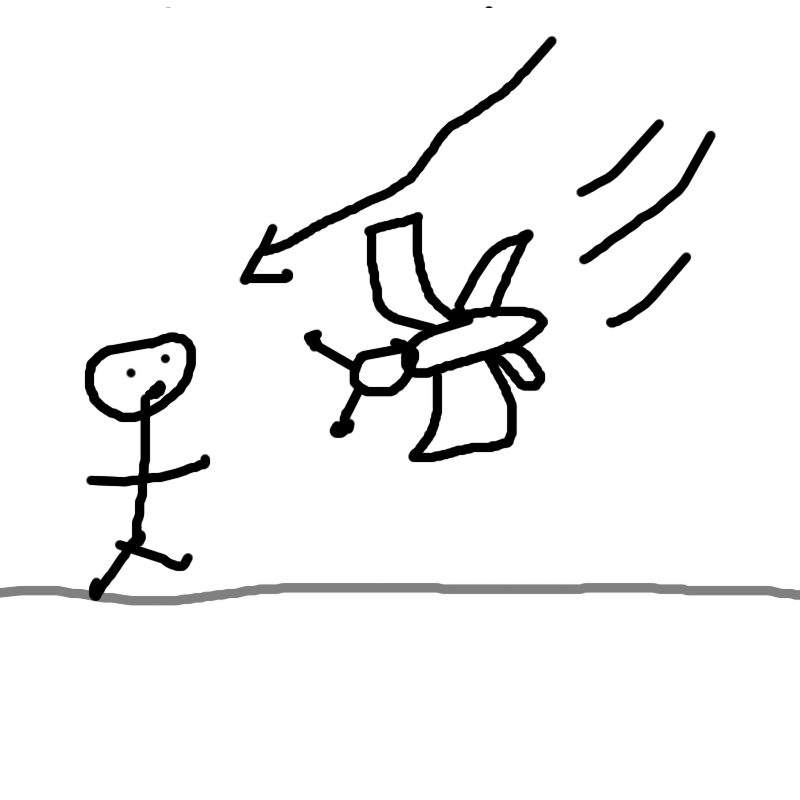
\includegraphics[height=0.2 \textheight]{Imagenes/embestidaA}
				\caption{Embestida aerea.}
				\label{fig:embestidaA}
			\end{figure}
%============================================================
\section{Nombre: Invisibilidad.} \label{hab.Invis}
\subsection{Descripción}
Esta habilidad le permite ser indetectable al ojo de dioses y humanos, permitiendole tomar una posición ventajosa en combate.
\subsection{Portador}
Itzpápalotl.
\subsection{Esquema}
			Ver figura \ref{fig:invisibilidad}.
			\begin{figure}
				\centering
				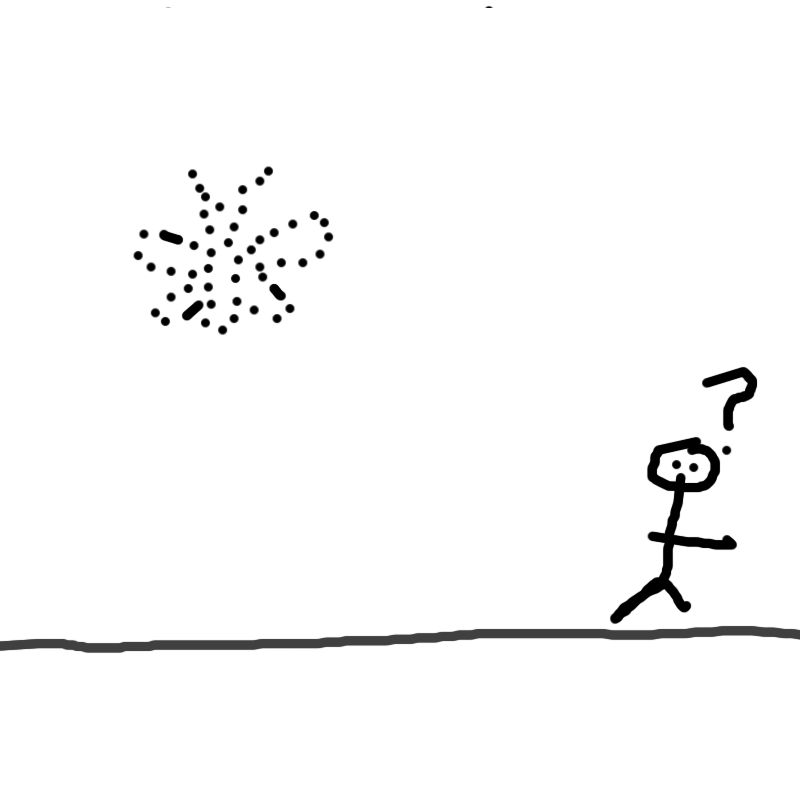
\includegraphics[height=0.2 \textheight]{Imagenes/invisibilidad}
				\caption{Invisibilidad.}
				\label{fig:invisibilidad}
			\end{figure}
%============================================================
\section{Nombre: Tornado.} \label{hab.tornado}
\subsection{Descripción}
Poderoso ataque que puede bajar hasta la mitad de la vida del jugador.
\subsection{Portador}
Mictlecayotl.
\subsection{Esquema}
			Ver figura \ref{fig:tornado}.
			\begin{figure}
				\centering
				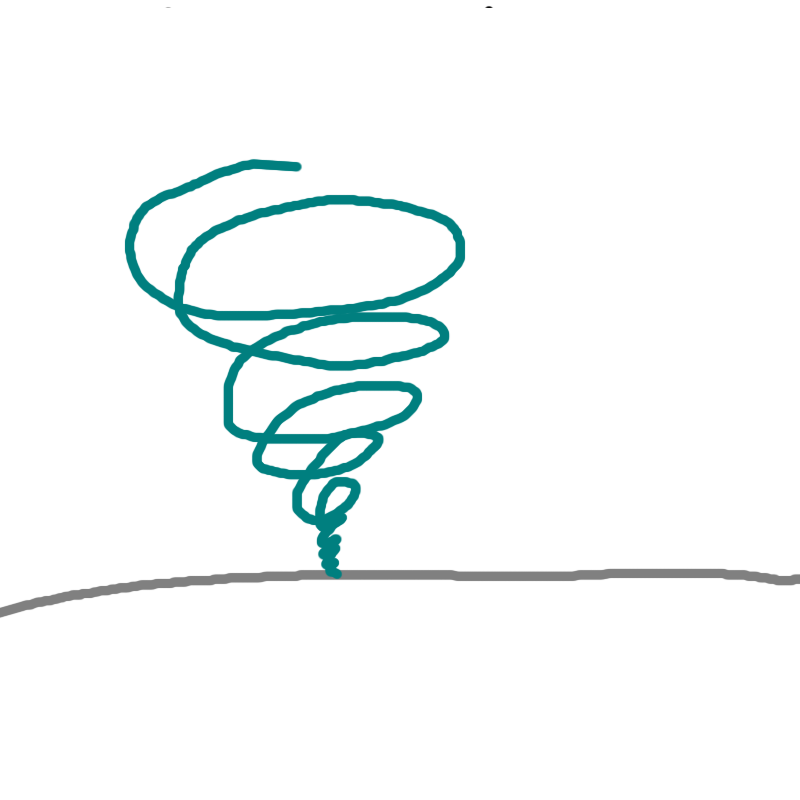
\includegraphics[height=0.2 \textheight]{Imagenes/tornado}
				\caption{Tornado.}
				\label{fig:tornado}
			\end{figure}

%============================================================
\section{Nombre: Ventisca.} \label{ventisca}
\subsection{Descripción}
Aire helado que puede causar una pérdida considerable de la barra de salud.
\subsection{Portador}
Mictlecayotl.
\subsection{Esquema}
			Ver figura \ref{fig:ventisca}.
			\begin{figure}
				\centering
				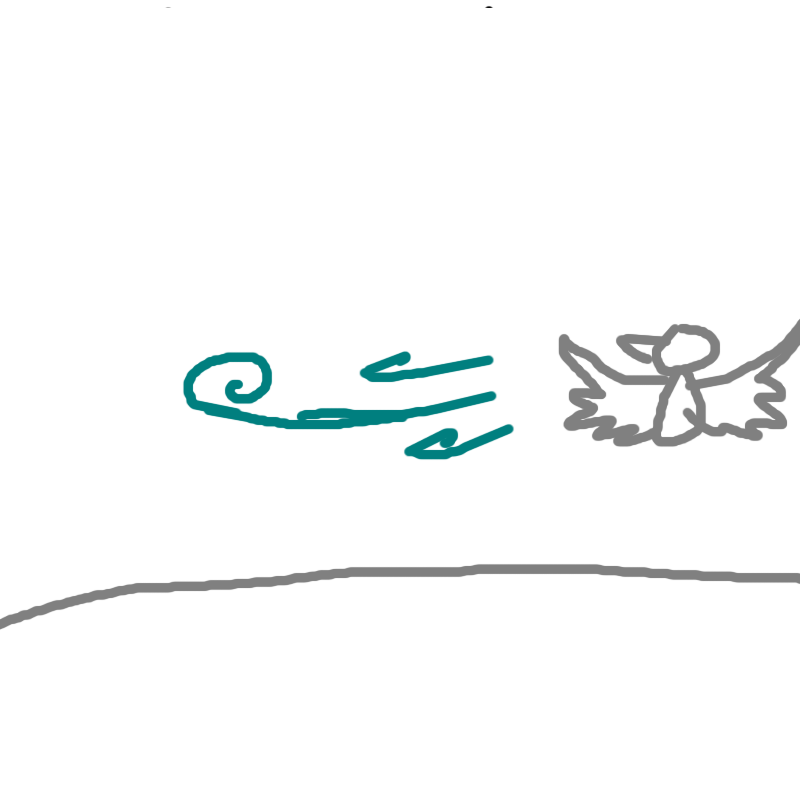
\includegraphics[height=0.2 \textheight]{Imagenes/ventisca}
				\caption{Ventisca.}
				\label{fig:ventisca}
			\end{figure}

%============================================================
\section{Nombre: Raíz del diablo.}\label{hab.RaizDia}
\subsection{Descripción}
Ataque que produce una confusión en el jugador, haciendo que los botones no reaccionen con las acciones que deberían.
\subsection{Portador}
Tlazoltéotl.
\subsection{Esquema}
			Ver figura \ref{fig:raiz}.
			\begin{figure}
				\centering
				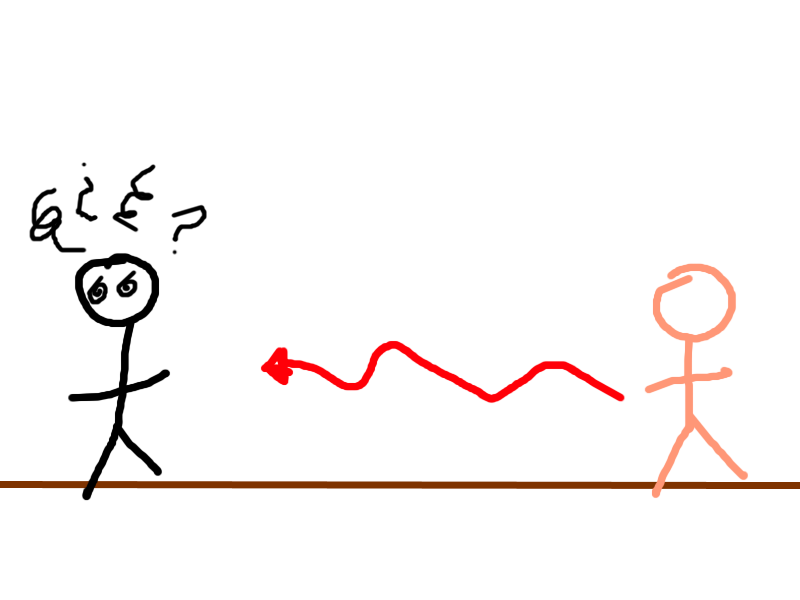
\includegraphics[height=0.2 \textheight]{Imagenes/raiz}
				\caption{Raíz del diablo.}
				\label{fig:raiz}
			\end{figure}

%============================================================
\section{Nombre: Energía corrupta.} \label{hab.CorrupEner}
\subsection{Descripción}
Esferas de energia oscura que infringen daño al jugador al hacer contacto con éste.
\subsection{Portador}
Tlazoltéotl.
\subsection{Esquema}
			Ver figura \ref{fig:energiaC}.
			\begin{figure}
				\centering
				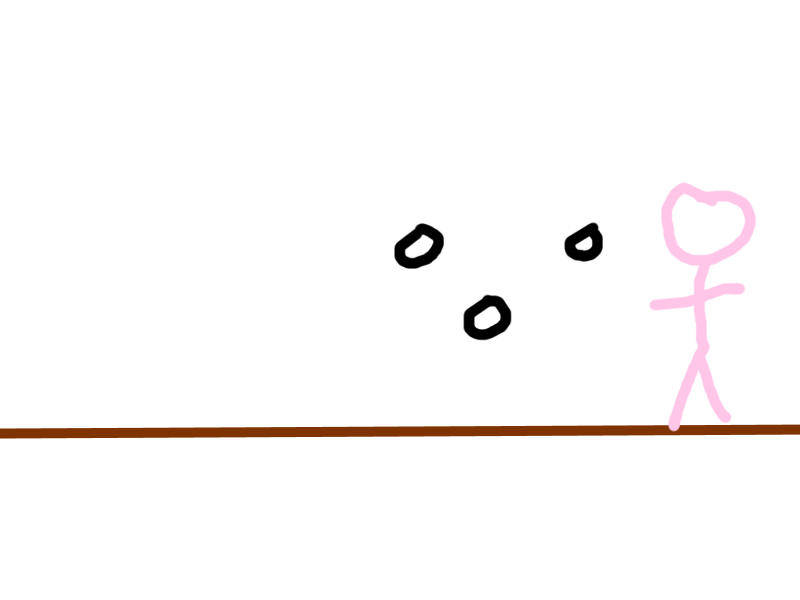
\includegraphics[height=0.2 \textheight]{Imagenes/energiaC}
				\caption{Energía corrupta.}
				\label{fig:energiaC}
			\end{figure}	

%============================================================
\section{Nombre: Circulo protector.} \label{hab.CirPro}
\subsection{Descripción}
Utilizando energía corrupta,  Tlazoltéotl crea alrededor de ella un circulo con la capacidad de protegerla contra cualquier ataque.
\subsection{Portador}
Tlazoltéotl.
\subsection{Esquema}
			Ver figura \ref{fig:circuloP}.
			\begin{figure}
				\centering
				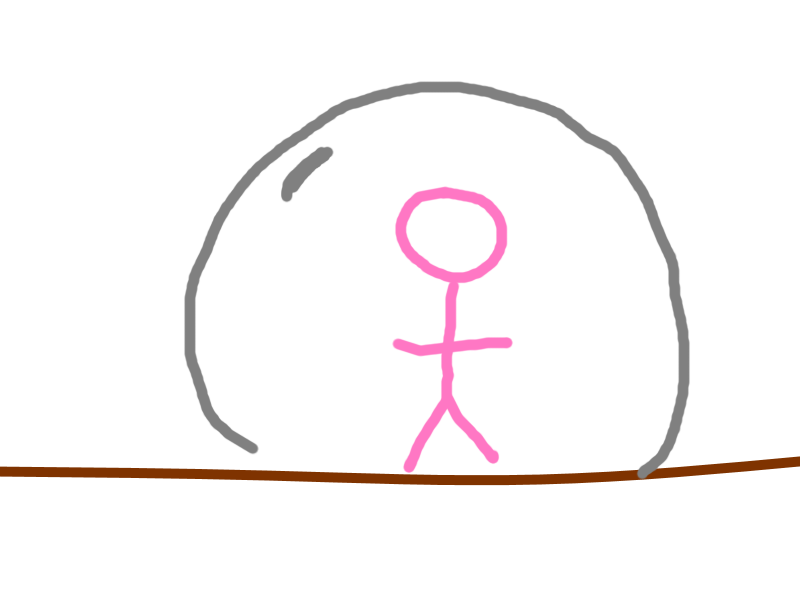
\includegraphics[height=0.2 \textheight]{Imagenes/circuloP}
				\caption{Círculo protector.}
				\label{fig:circuloP}
			\end{figure}

%============================================================
\section{Nombre: LLuvia de lava.} \label{hab.LLuviaLava}
\subsection{Descripción}
Caen bolas de lava con una gran capacidad de daño.
\subsection{Portador}
Itztlacoliuhqui.	
\subsection{Esquema}	
			Ver figura \ref{fig:lluviaL}.
			\begin{figure}
				\centering
				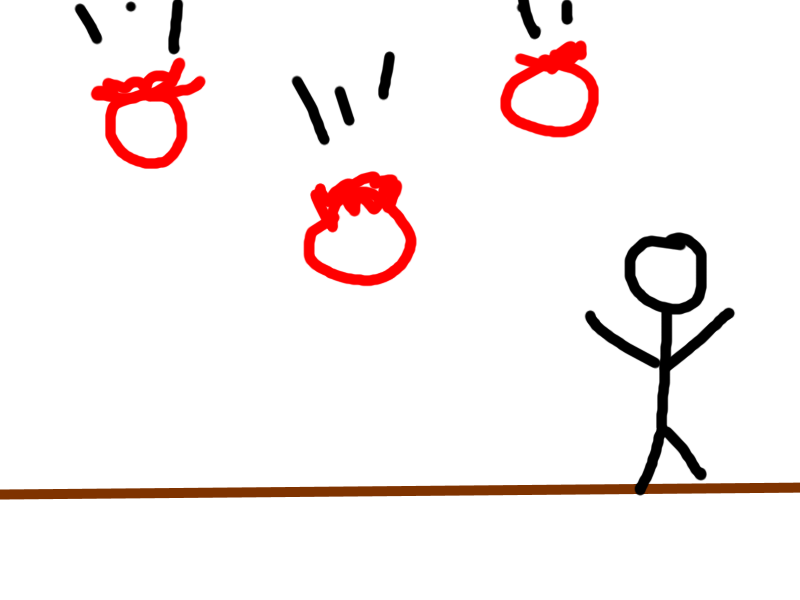
\includegraphics[height=0.2 \textheight]{Imagenes/lluviaL}
				\caption{Lluvia de lava.}
				\label{fig:lluviaL}
			\end{figure}

%============================================================
\section{Nombre: Manotazo.} \label{hab.Manotazo}
\subsection{Descripción}
Genera una onda expansiva que deforma el suelo provonado una oleada de rocas.
\subsection{Portador}
\subsection{Esquema}
			Ver figura \ref{fig:manotazo}.
			\begin{figure}
				\centering
				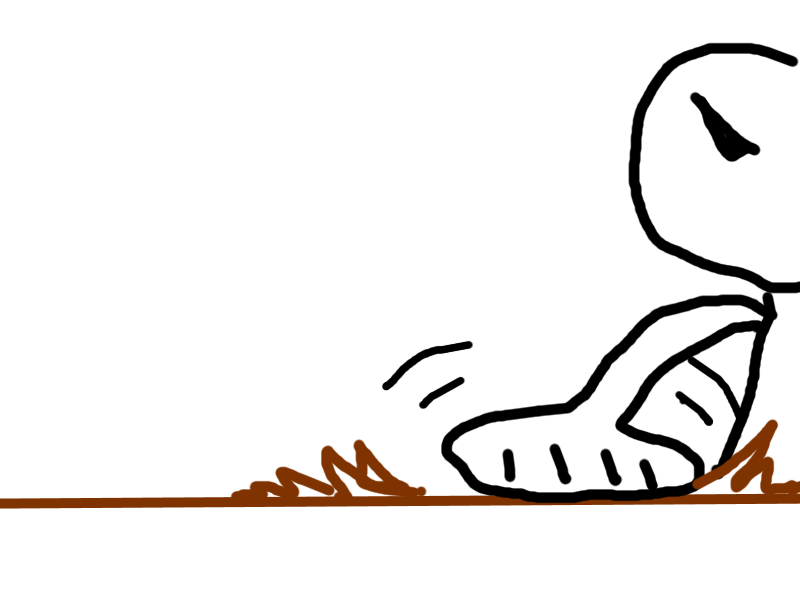
\includegraphics[height=0.2 \textheight]{Imagenes/manotazo}
				\caption{Manotazo.}
				\label{fig:manotazo}
			\end{figure}
Itztlacoliuhqui.

%============================================================
\section{Nombre: Lluvia de flechas.} \label{hab.LluviaFle}
\subsection{Descripción}
Como su nombre lo dice, provoca una lluvia de flechas, este es el ataque de Itztlacoliuhqui que genera el menor nivel de daño. 
\subsection{Portador}
Itztlacoliuhqui.
\subsection{Esquema}
			Ver figura \ref{fig:lluviaF}.

%============================================================
\section{Nombre: Todos los hombres del rey.}\label{hab.TodoRey}
\subsection{Descripción}
Con este ataque,  Mictlantechtli invoca a varios de los enemigos normales que habitan el Mictlán para que se enfrenten al jugador mientras  Mictlantechhtli desaparece.
\subsection{Portador}
Mictlantechtli.
\subsection{Esquema}
			Ver figura \ref{fig:rey}.
			\begin{figure}
				\centering
				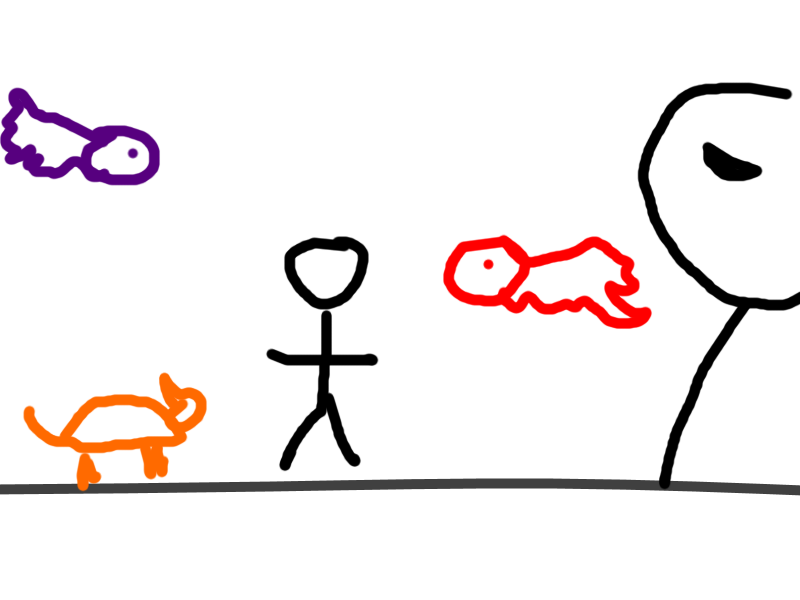
\includegraphics[height=0.2 \textheight]{Imagenes/rey}
				\caption{Todos los hombres del rey.}
				\label{fig:rey}
			\end{figure}
%============================================================
\section{Nombre: Fuego mortífero.} \label{hab.FuegoMor}
\subsection{Descripción}
Mictlantechtli  lanza poderosas esferas de fuego verde.
\subsection{Portador}
Mictlantechtli.	
\subsection{Esquema}	
			Ver figura \ref{fig:fuegoM}.
			\begin{figure}
				\centering
				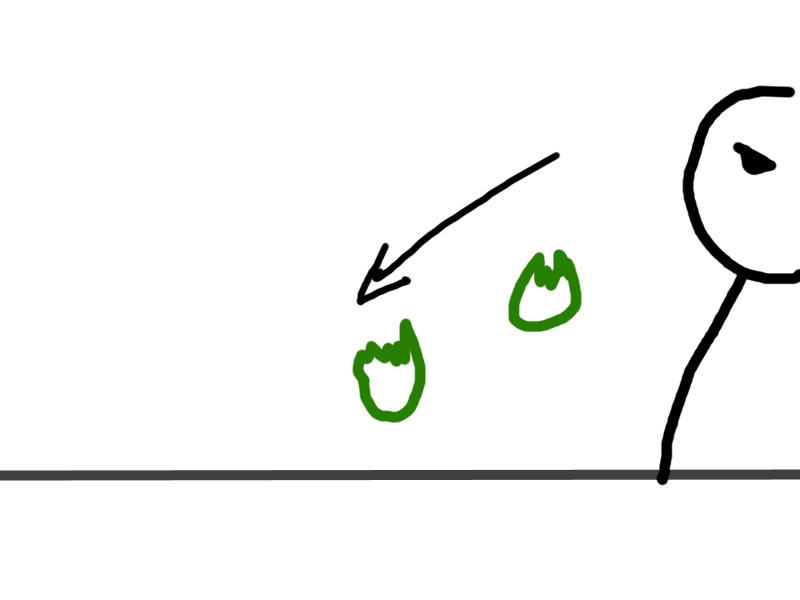
\includegraphics[height=0.2 \textheight]{Imagenes/fuegoM}
				\caption{fuegoM.}
				\label{fig:fuegoM}
			\end{figure}
%============================================================
\section{Nombre: Penitencia.}\label{hab.Penitencia}
\subsection{Descripción}
Mictlantechtli se eleva en el aire haciendo que salgan huesos filosos del suelo.
\subsection{Portador}
Mictlantechtli.
\subsection{Esquema}
			Ver figura \ref{fig:penitencia}.
			\begin{figure}
				\centering
				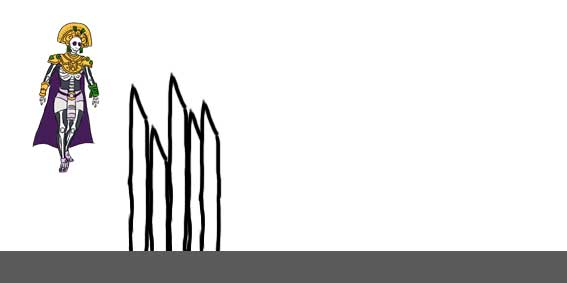
\includegraphics[height=0.2 \textheight]{Imagenes/penitencia}
				\caption{Penitencia.}
				\label{fig:penitencia}
			\end{figure}

